\documentclass[11pt]{article}

% ====================================================
% ====================================================
% USEPACKAGES AND IMPORTS
% ====================================================
% ====================================================

\usepackage[T1]{fontenc}
\usepackage[utf8]{inputenc}
\usepackage[english]{babel}

\usepackage{tikz}
\usepackage{eso-pic}
\usepackage{fancyhdr}
\usepackage{enumitem}
\usepackage{amssymb}
\usepackage{roboto}
\renewcommand{\familydefault}{\sfdefault}

% definitions
% ====================================================
\let\titleoriginal\title
\renewcommand{\title}[1]{
	\titleoriginal{#1}
	\newcommand{\thetitle}{#1}
}

\setlength{\parskip}{\baselineskip}%
\setlength{\parindent}{0pt}%

\newcommand\exercise[3]{
	\item #1\vspace{0.2cm}\newline #2 \vspace{#3}
}

% header and footer
\pagestyle{fancy}
\fancyhf{}

\lhead{\thetitle}
\rhead{
\includegraphics[width=2cm]{../../img/logo_dhbw.png}}
\cfoot{\thepage\\\vspace{0.6cm} \small Applied Machine Learning Fundamentals}

\setlength{\headsep}{1.5cm}

% title page theme
\newcommand\BackgroundPic{%
\put(0,0){%
\parbox[b][\paperheight]{\paperwidth}{%
\vfill
\centering
\tikz[overlay,remember picture] \node[opacity=0.2, at=(current page.center)] {
	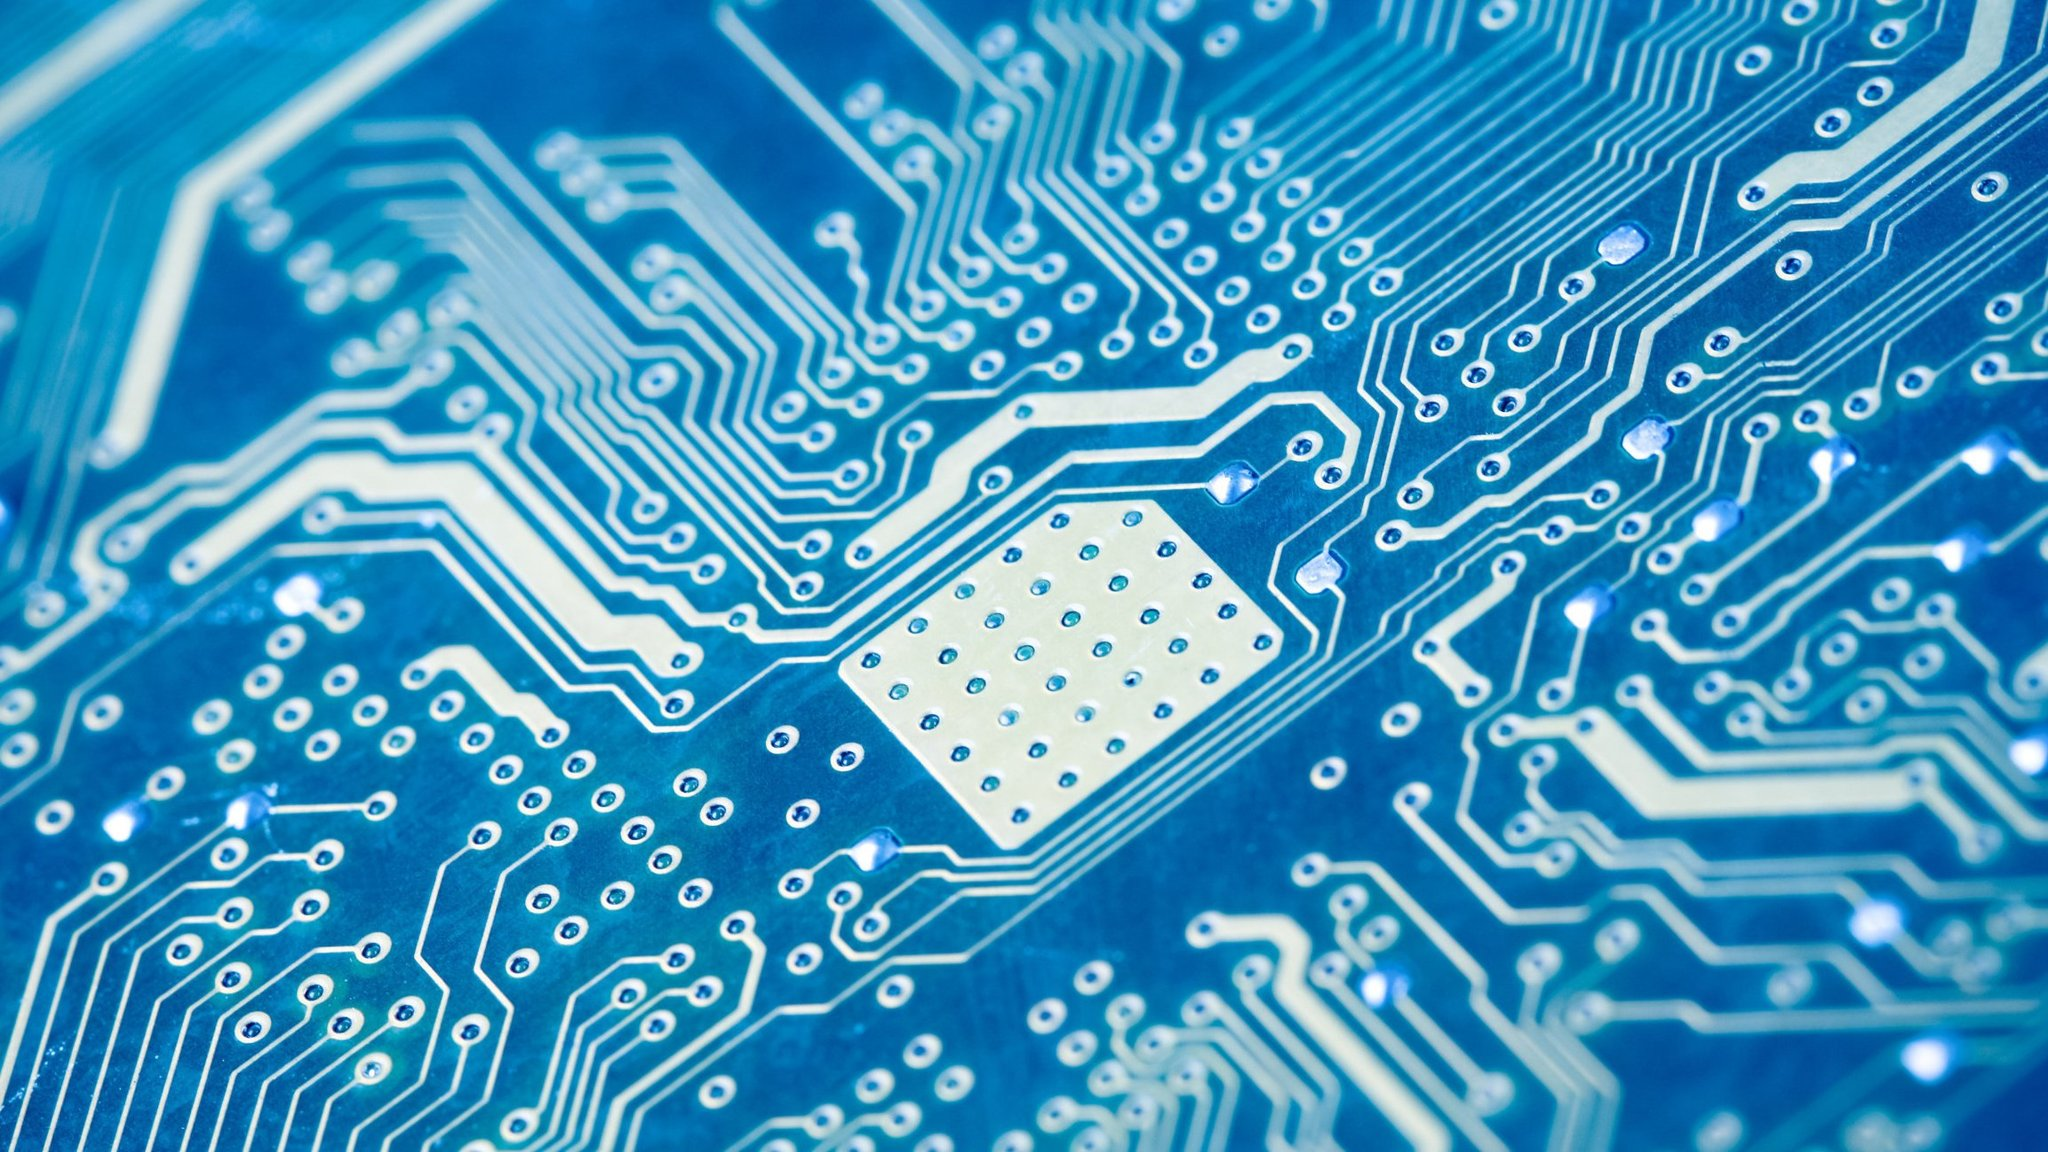
\includegraphics[height=\paperheight,width=\paperwidth]{../../img/processor.jpg}
};

\includegraphics[width=4cm, trim=-5.5cm 0 0 -1cm]{../../img/logo_dhbw.png}
%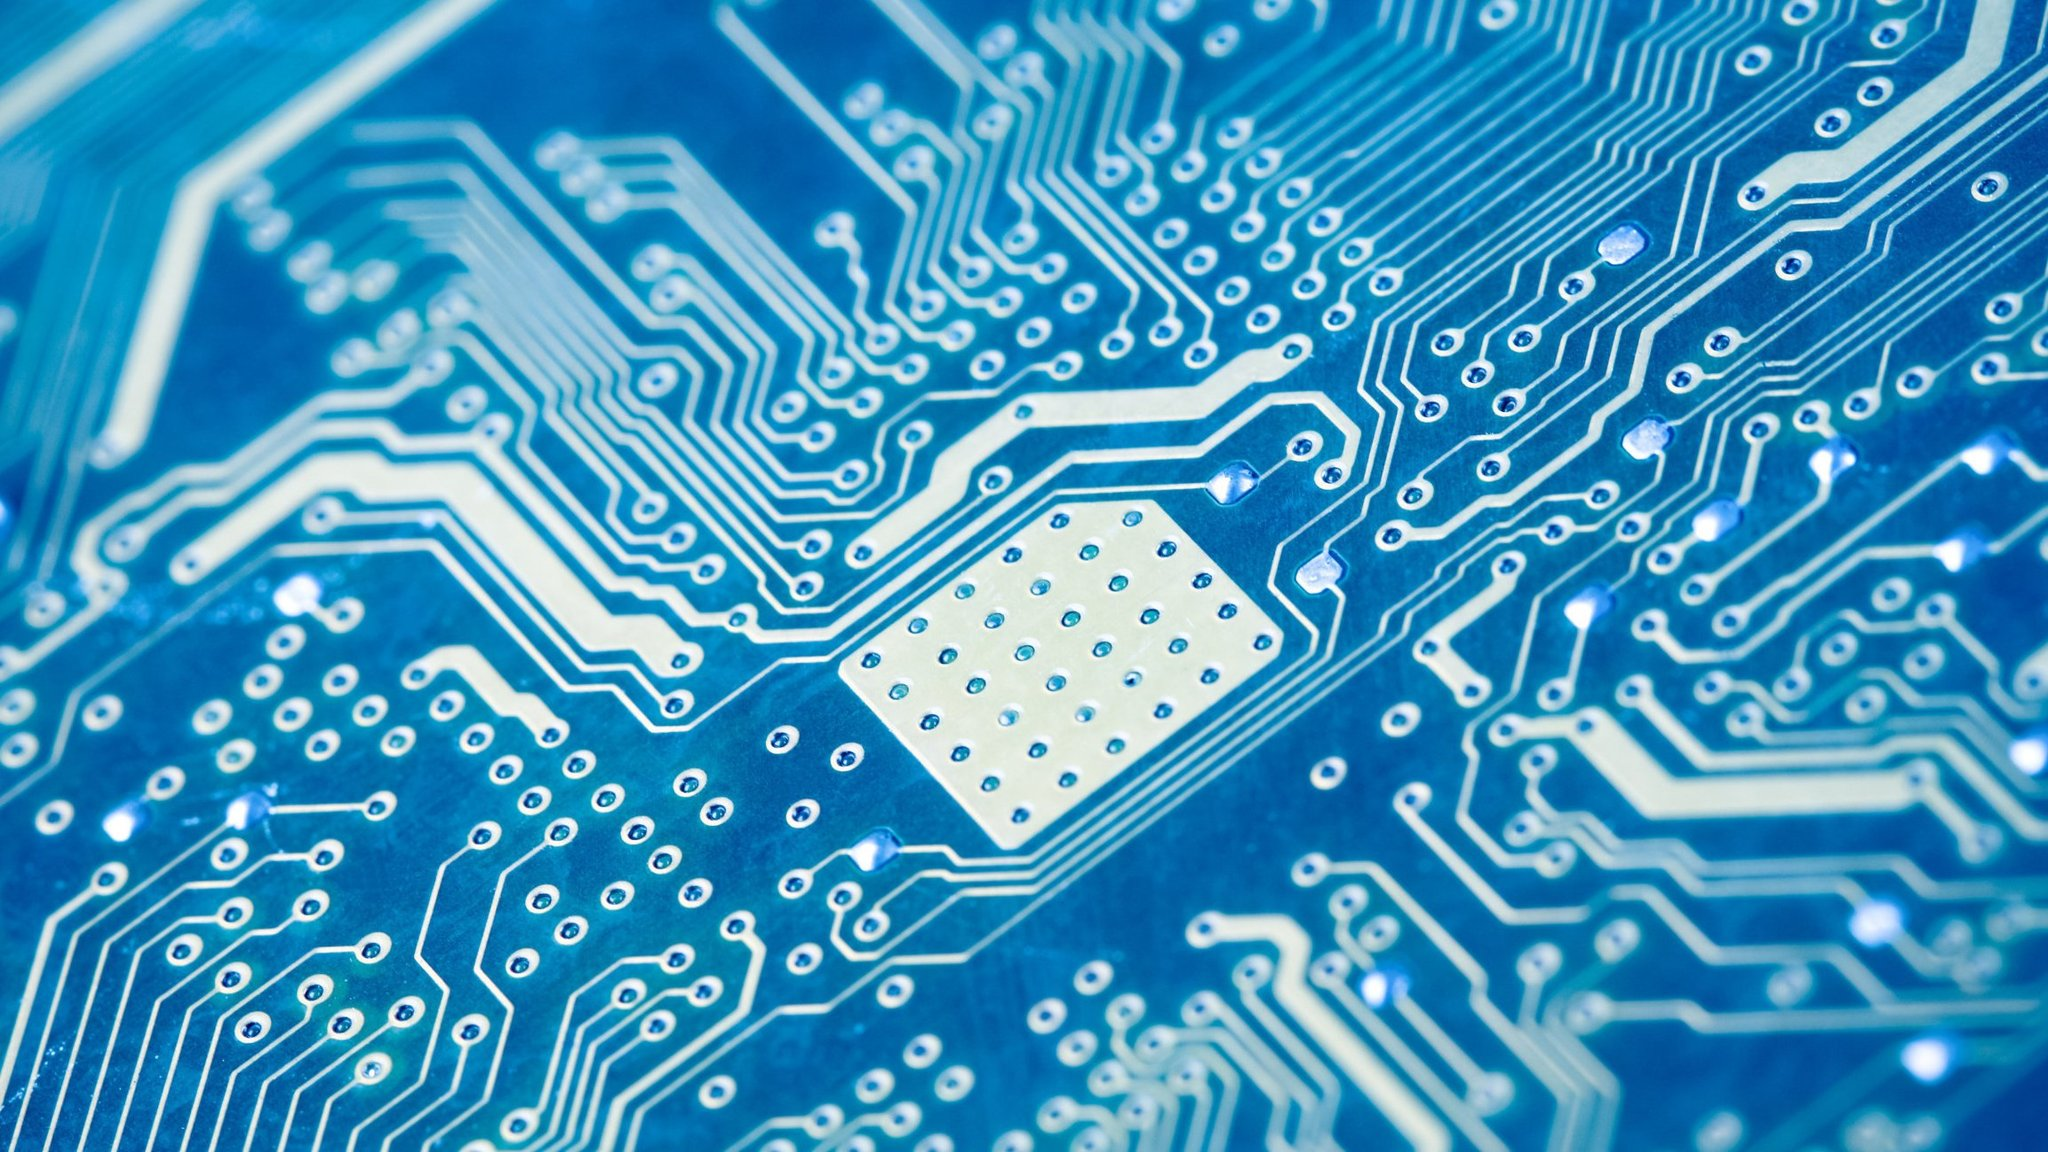
\includegraphics[width=\paperwidth,height=\paperheight,%
%keepaspectratio]{../../img/processor.jpg}%
\vfill
}}}
